\documentclass[a4paper,12pt]{article}

\usepackage[T2A]{fontenc}			
\usepackage[utf8]{inputenc}			
\usepackage[english,russian]{babel}	

\usepackage[
bookmarks=true, colorlinks=true, unicode=true,
urlcolor=black,linkcolor=black, anchorcolor=black,
citecolor=black, menucolor=black, filecolor=black,
]{hyperref}

\usepackage{color}
\usepackage{caption}
\DeclareCaptionFont{white}{\color{black}}
\DeclareCaptionFormat{listing}{\colorbox{white}{\parbox{\textwidth}{#1#2#3}}}
\captionsetup[lstlisting]{format=listing,labelfont=white,textfont=white}

\usepackage{amsmath,amsfonts,amssymb,amsthm,mathtools} 
\usepackage{wasysym}

\usepackage{graphicx}
%\usepackage[cache=false]{minted}
\usepackage{cmap}
\usepackage{indentfirst}

\usepackage{listings} 
\usepackage{fancyvrb}

\usepackage{geometry}
\geometry{left=2cm}
\geometry{right=1.5cm}
\geometry{top=1cm}
\geometry{bottom=2cm}

\usepackage[cache=false]{minted}

\setlength{\parindent}{5ex}
\setlength{\parskip}{0.5em}

\usepackage{longtable}

\usepackage{pgfplots}
\usetikzlibrary{datavisualization}
\usetikzlibrary{datavisualization.formats.functions}

\begin{document}

	\lstset{ %
		language=C,                 % выбор языка для подсветки (здесь это С)
		basicstyle=\small\sffamily, % размер и начертание шрифта для подсветки кода
		numbers=left,               % где поставить нумерацию строк (слева\справа)
		numberstyle=\tiny,           % размер шрифта для номеров строк
		stepnumber=1,                   % размер шага между двумя номерами строк
		numbersep=5pt,                % как далеко отстоят номера строк от подсвечиваемого кода
		backgroundcolor=\color{white}, % цвет фона подсветки - используем \usepackage{color}
		showspaces=false,            % показывать или нет пробелы специальными отступами
		showstringspaces=false,      % показывать или нет пробелы в строках
		showtabs=false,             % показывать или нет табуляцию в строках
		frame=single,              % рисовать рамку вокруг кода
		tabsize=2,                 % размер табуляции по умолчанию равен 2 пробелам
		captionpos=t,              % позиция заголовка вверху [t] или внизу [b] 
		breaklines=true,           % автоматически переносить строки (да\нет)
		breakatwhitespace=false, % переносить строки только если есть пробел
		escapeinside={\%*}{*)}   % если нужно добавить комментарии в коде
	}

	\vspace*{30mm} 
	
	{\huge
	\begin{center}
		КР№2 по экологии
	\end{center}

	
	
	\begin{center}
		группа: ИУ7-62Б
	\end{center}

	
	
	\begin{center}
		Левушкин Илья Кириллович
	\end{center}

	
	
	\begin{center}
		Вариант: 9
	\end{center}
}

	\newpage
	
	\section*{Задание №1}
	
	Сравнить два вида электростанций по основным экологическим и
	эксплуатационным характеристикам (вспомните лекцию) по вариантам.
	
	Привести по одному примеру каждой из двух ЭС (с фото, указанием
	местоположения и суммарной установленной/номинальной мощности: т. е. если
	у вас вместе 10 ветряков, то указываем суммарную мощность 10 ветряков).
	
	Расшифровка сокращений:
	
	ТЭС — тепловые электростанции (например, работающие на угле);
	
	АЭС — атомные электростанции;
	
	ГЭС — гидроэлектростанции (не берём в расчёт малые ГЭС);
	
	ВЭС — ветряные электростанции;
	
	СЭС — солнечные электростанции;
	
	ГеотЭС — геотермальные электростанции.
	
	ЭС по варианту: АЭС, ТЭС
	
	
	\section*{Сравнение ТЭС и АЭС по основным экологическим характеристикам}
	
	\subsection*{Пример ТЭС}
	
	{\bf Череповецкая ГРЭС}
	
	\begin{figure}[h!]
		\begin{center}
			{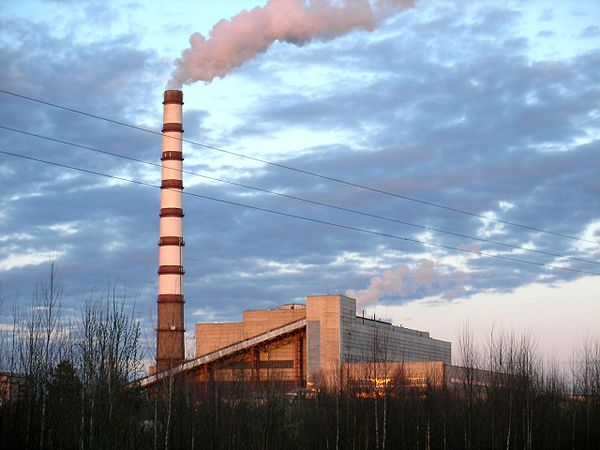
\includegraphics[scale = 0.6]{gres.jpg}}
			\label{ГРЭС}
		\end{center}
		\caption{Череповецкая ГРЭС}
	\end{figure}
	
	\newpage

	{\bf Местоположение} -- поселок Кадуй, Вологодская область, Россия
	
	{\bf Электрическая мощность} -- 1080 МВт.
	
	{\bf Основное топливо} -- природный газ, уголь.
	
	{\bf Резервное топливо} -- мазут.
	
	\subsection*{Пример АЭС}
	
	
	{\bf ВВЭР-1000}
	
	\begin{figure}[h!]
		\begin{center}
			{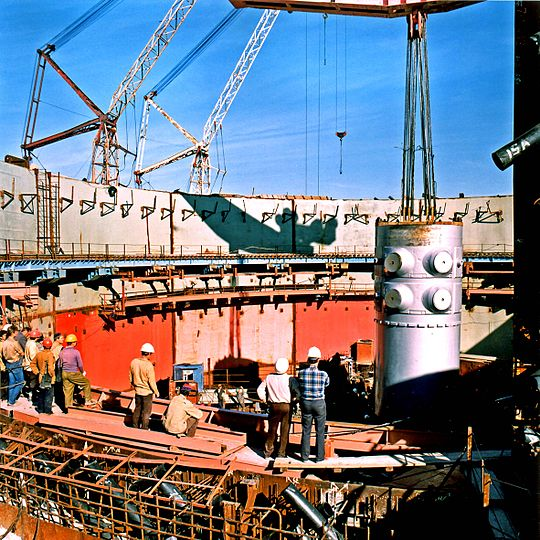
\includegraphics[scale = 2.0]{AES.jpg}}
			\label{AES}
		\end{center}
		\caption{ВВЭР-1000}
	\end{figure}
	
	{\bf Местоположение} -- Блок-5 НВАЭС, Воронежская область, Нововоронеж, Россия.
	
	{\bf Электрическая мощность} -- 1000 МВт.
	
	{\bf Топливо} -- Диоксид урана.
	
	\newpage
	
	\subsection*{Экологическая характеристика}
	
	Ниже приведена таблица основных экологических характеристик для угольной ТЭС и Атомной ЭС  мощностью 1000 МВт.
	
	\begin{center}
		\begin{longtable}[h!]{|p{0.45\linewidth}|p{0.25\linewidth}|p{ 0.25\linewidth}|}
			\hline
			{Потребление топлива и выбросы в год} & {ТЭС} & {АЭС}\\
			\hline
			{1. Потребление топлива (в тоннах)} & {3,9 млрд} & {30}\\
			\hline
			{Потребление атмосферного кислорода (м$^3$)} & {5,5 млрд} & {нет}\\
			\hline
			{3. Газовые выбросы (в тоннах)} & {} & {}\\
			\hline
			{Углекислый газ} & {10 млн} & {нет}\\
			\hline
			{Окислы серы} & {124 тыс} & {нет}\\
			\hline
			{Окислы азота} & {34 тыс} & {нет}\\
			\hline
			{4. Выбросы неуловимой золы (в тоннах)} & {7,3 тыс} & {нет}\\
			\hline
			{5. Канцерогенные вещества (в тоннах)} & {0, 012} & {нет}\\
			\hline
			{6. Пятиокись ванадия (в тоннах)} & {37} & {нет}\\
			\hline
			{7. Твердые отходы (в тоннах)} & {80 тыс} & {нет}\\
			\hline
		\end{longtable}
	\end{center}

	Согласно таблице, атомные ЭС при нормальной работе практически не загрязняют окружающую среду в сравнении с угольной ТЭС. Однако, аварии на атомных станциях влекут за собой гораздо более опасные экологические последствия нежели при авариях на ТЭС.
	
	Радиоактивное загрязнение с помощью воздушных течений и вод распространяются на территории весьма удаленные от АЭС. Так, на Чернобыльской АЭС высота выбросов из аварийного блока достигла 1200 м. Отсюда мощными воздушными течениями радионуклиды распространились на многие тысячи километров.
	
	\section*{Эксплуатационная характеристика}
	
	
	\begin{center}
		\begin{longtable}[h!]{|p{0.45\linewidth}|p{0.25\linewidth}|p{ 0.25\linewidth}|}
			\hline
			{Типы электростанций} & {Удельные
			
		капиталовложения, р./кВт} & {Себестоимость
	
производства энергии, коп./кВт*ч}\\
			\hline
			{Газовая ЭС} & {1500} & {12-15}\\
			\hline
			{АЭС} & {2000-3000} & {12-15}\\
			\hline
		\end{longtable}
	\end{center}

	Видно, что удельные капиталовложения в АЭС в среднем превосходят в 1.5-2 раза в газовую ЭС.
	
	\section*{Задание №2}
	
	Подготовить краткое сообщение по глобальной экологической проблеме
	(по варианту) по следующему плану:
	
	\begin{enumerate}
		\item описать суть проблемы, привести численные данные (с указанием
		ссылок);
		\item основные антропогенные причины, вызывающие её (её негативные
		проявления);
		\item последствия проблемы;
		\item мероприятия, принимаемые на международном и национальном уровнях:
		
		\begin{enumerate}
			\item общие сведения, что делать/не делать для улучшения ситуации;
			\item принятые международные конвенции, протоколы, соглашения... (с
			указанием ссылок на текст действующей редакции на русском или
			английском языках);
			\item действующие законы, программы, мероприятия в стране (иностранцы
			про свои страны пишут; остальные — про Россию и регион, выбранный
			для презентации);
		\end{enumerate}
		\item тенденции развития проблемы, результаты предпринятых мероприятий
	\end{enumerate}

	Глобальная экологическая проблема по варианту: <<Космический мусор>>.
	
	\section*{Космический мусор}
	
	\subsection*{Суть проблемы}
	
	В настоящее время в районе низких околоземных орбит вплоть до высот около 2000 км находится, по разным оценкам, порядка 300 тыс. техногенных объектов общей массой до 5000 тонн. (~\cite{OOH}). На основе статистических оценок делаются выводы, что общее число подобных объектов поперечником более 1 см достаточно неопределенно и может достигать 60 000—100 000.
	
	
	
	\subsection*{Основные антропогенные причины}
	
	Запуски ракет, разрушение и падение фрагментов космических аппаратов образуют космический мусор на орбите нашей планеты и приводят к серьезным экологическим проблемам на Земле и в космосе.
	
	\subsection*{Последствия проблемы}
	
	Космический мусор может привести к прекращению всякой деятельности в космосе, поскольку имеет свойство саморазмножаться — крупные обломки аппаратов, сталкиваясь между собой, порождают многочисленное <<население>> более мелкого мусора.
	
	\subsection*{Мероприятия, принимаемые на международном и национальном уровнях}
	
	Эффективных практических мер по уничтожению космического мусора на орбитах более 600 км на настоящем уровне технического развития человечества пока не разработано.
	
	Хотя были проекты спутников, испаряющих обломки мощным лазерным лучом (~\cite{1}) или меняющих их орбиту ионными пучками (~\cite{2}, ~\cite{3}) , которые должны тормозить обломки для их входа в атмосферу с частичным или полным сгоранием в ней или, в случае аппаратов на геостационарной орбите, уводить их на орбиту захоронения, или наземные лазеры (~\cite{4}, ~\cite{5}).
	
	На данный момент в России разрабатывается проект космического аппарата для сбора мусора на орбите Земли  (~\cite{6}).
	
	\subsection*{Тенденции развития проблемы}

	Как уже было сказано, на данный момент эффективных практических мер по уничтожению космического мусора пока не разработано, поэтому происходит только усугубление проблемы со временем. Всего за последние 30 лет количество мусора на орбите земли более чем удвоилось.

	\pagebreak
	
	\addcontentsline{toc}{section}{Список литературы}
	\begin{thebibliography}{}
		
		\bibitem{OOH}
		Доклад Научно-технического подкомитета о работе
		его сорок шестой сессии, проведенной в Вене
		9-20 февраля 2009 года
		[Электронный ресурс]. – Режим доступа: 
		https://www.unoosa.org/pdf/reports/ac105/AC105\_933R.pdf, свободный – 
		(25.05.2020)
		
		\bibitem{1}
		Assessment Study of Small Space Debris Removal by Laser Satellites
		[Электронный ресурс]. – Режим доступа: 
		http://ntrs.nasa.gov/archive/nasa/casi.ntrs.nasa.gov/20120009369.pdf, свободный – 
		(25.05.2020)
		\bibitem{2}
		Ion Beam Shepherd for Contactless Space Debris Removal
		[Электронный ресурс]. – Режим доступа: 
		https://arxiv.org/pdf/1102.1289.pdf, свободный – 
		(25.05.2020)
		\bibitem{3}
		Пространственное движение цилиндрического космического мусора при его уборке
		ионным потоком
		[Электронный ресурс]. – Режим доступа: 
		http://www.ledkov.ru/papers/MPE2017\_rus.pdf, свободный – 
		(25.05.2020)
		\bibitem{4}
		The Independent
		[Электронный ресурс]. – Режим доступа: 
		https://www.independent.co.uk/news/science/space-debris-orbiting-earth-to-be-targeted-with-giant-lasers-fired-from-australia-9181280.html, свободный – 
		(25.05.2020)
		\bibitem{5}
		MIT Technology Review
		[Электронный ресурс]. – Режим доступа: 
		https://www.technologyreview.com/view/423302/nasa-studies-laser-for-removing-space-junk/, свободный – 
		(25.05.2020)
		\bibitem{6}
		Ученые РКС представили проект спутника-охотника на космический мусор
		[Электронный ресурс]. – Режим доступа: 
		http://russianspacesystems.ru/2019/03/27/uchenye-rks-predstavili-proekt-sputnika/, свободный – 
		(25.05.2020)
	\end{thebibliography}

\end{document}